%%%%%%%%%%%%%%%%%%%%%%%%%%%%%%%%%%%%%%%%%
% Lachaise Assignment
% LaTeX Template
% Version 1.0 (26/6/2018)
%
% This template originates from:
% http://www.LaTeXTemplates.com
%
% Authors:
% Marion Lachaise & François Févotte
% Vel (vel@LaTeXTemplates.com)
%
% License:
% CC BY-NC-SA 3.0 (http://creativecommons.org/licenses/by-nc-sa/3.0/)
% 
%%%%%%%%%%%%%%%%%%%%%%%%%%%%%%%%%%%%%%%%%

%----------------------------------------------------------------------------------------
%	PACKAGES AND OTHER DOCUMENT CONFIGURATIONS
%----------------------------------------------------------------------------------------

\documentclass[bibnotes]{article}
\usepackage{hyperref}
\usepackage{caption}
\usepackage{subcaption}
\usepackage{mathtools}
\usepackage{natbib}
\usepackage{physics}
\usepackage{amsmath}

% \usepackage{subfig}
\input{structure.tex} % Include the file specifying the document structure and custom commands

%----------------------------------------------------------------------------------------
%	ASSIGNMENT INFORMATION
%----------------------------------------------------------------------------------------

\DeclareMathOperator{\re}{Re}
\DeclareMathOperator{\im}{Im}
\DeclareMathOperator{\sign}{sign}

\newcommand{\SLJ}[3]{{\ensuremath{{^{#1}}\mathrm{#2}_{#3}}}}
\newcommand{\TPT}{\SLJ{3}{P}{2}}
\newcommand{\TPO}{\SLJ{3}{P}{1}}
\newcommand{\TPZ}{\SLJ{3}{P}{0} \ }
\newcommand{\TPJ}{\SLJ{3}{P}{J}}
\newcommand{\TSO}{\SLJ{3}{S}{1}}
\newcommand{\SSZ}{\SLJ{1}{S}{0} \ }
\newcommand{\SPO}{\SLJ{1}{P}{1}}
\newcommand{\TDO}{\SLJ{3}{D}{1}}
\newcommand{\SDT}{\SLJ{1}{D}{2}}

\newcommand{\Isotope}[2]{\ensuremath{^{{#1}}\text{{#2}}}\xspace}
\newcommand{\Sr}[1]{\Isotope{{#1}}{Sr}}

\title{Cavity Ring Project Data Analysis} % Title of the assignment

\author{Annie Jihyun Park\\ \texttt{ajpark@mpq.mpg.de}} % Author name and email address

\date{\today} % University, school and/or department name(s) and a date

%----------------------------------------------------------------------------------------

\begin{document}

\maketitle % Print the title

%----------------------------------------------------------------------------------------
%	INTRODUCTION
%----------------------------------------------------------------------------------------

\section*{Introduction} % Unnumbered section

	We use the spatially dependent ac-Stark shift of the clock transition to map the intensity profile of the cavity lattices. This document summarizes the data analysis went into the cavity fringe project. 

% The focus of our paper will be about integrating the build-up cavities for optical lattice experiments, demonstrating its viability to create high contrast, large, homogeneous, and deep optical lattices in a stable and compact way.
% The Gaussian intensity profile of optical lattices is one of the central features that characterizes the homogeneity and size of the lattices. For this reason, 
% For this reason, we chose the lattice wavelength to be 914 nm to maximize the stark shift, whereas the sheet beam wavelength is magic, 813 nm, to eliminate the influence of the sheet light. 
%----------------------------------------------------------------------------------------
%	PROBLEM 1
%----------------------------------------------------------------------------------------
\tableofcontents

\section{Clock excitation}
\label{sec:clock excitation}

\subsection{Clock excitation without dephasing}

	The clock transition \SSZ $\leftrightarrow$ \TPZ is forbidden in even isotopes of alkaline-earth atoms due to the absence of hyperfine mixing (nuclear spin $I$=0). However, with a small external magnetic field, it is possible to induce the single-photon clock excitation by mixing \TPZ and \SSZ states (~\cite{Taichenachev06}, Figure \ref{fig:energy_level}):
	%
	\begin{align}
	\ket{\TPZ'}=\ket{\TPZ}+\frac{\Omega_{B}}{\Delta_{32}}\ket{\TPO}.
	\end{align}
	%
	\begin{figure}[h]
	    \centering
	    \includegraphics[scale=0.8]{figures/clock/energy_level}
	    \caption{(Adopted from ~\cite{Taichenachev06}) A small magnetic field breaks the LS coupling regime, and mixes \TPO ($\ket{3}$) \ and \TPZ($\ket{2}$) states, allowing otherwise forbidden transition from \SSZ to \TPZ.}
	    \label{fig:energy_level}
	\end{figure}
	%
	From~\cite{Taichenachev06}, the rabi frequency $\Omega$ for the \Sr{88} clock excitation is given by
	%
	\begin{align}
	\Omega&=\bra{\TPZ'}\mathbf{\hat{d}\cdot E}\ket{\SSZ}/\hbar=\frac{\Omega_L\Omega_B}{\Delta_{32}}\\
	&=\frac{\bra{\TPO}\mathbf{\hat{\mu}\cdot B}\ket{\TPZ}\bra{\TPO}\mathbf{\hat{d}\cdot E}\ket{\SSZ}}{\hbar^{2}\Delta_{32}}\\
	&=\frac{\langle\norm{\mu}\rangle\langle\norm{d}\rangle(\mathbf{E\cdot B)}} {\hbar^{2}\Delta_{32}}
	\end{align}
	%
	where $\langle\norm{\mu}\rangle$ and $\langle\norm{d}\rangle$ are reduced matrix elements. Using $\langle\norm{\mu}\rangle=\sqrt{2/3}\mu_{B}$ where $\mu_{B}$ is the Bohr magneton, $I=c\epsilon_{0}\abs{E}^{2}/2$, and $\langle\norm{d}\rangle$=0.151~\cite{cooper18}, the rabi frequency can be expressed in terms of the applied fields and light intensity
	%
	\begin{align}
		\Omega&=\alpha\sqrt{I}\abs{\textbf{B}}\text{cos}\theta
	\end{align}
	%
	\noindent where $\alpha$ is a measure of the induced Rabi frequency per unit of each of the fields, and $I$ is the light intensity, $\theta$ is the angle between linearly polarized $E$ and $B$ fields. Alternatively, $\Omega$ can be expressed in terms of the induced field shifts, the quadratic Zeeman $\Delta_B=\beta \textbf{B}^{2}$ and optical Stark $\Delta_L=\kappa I$ shifts where $\beta$ and $\kappa$ are respective shift coefficients, as 
	%
	\begin{align}
		\Omega=\xi\sqrt{\abs{\Delta_L \Delta_B}}\text{cos}\theta
	\end{align}
	%
	where $\xi\equiv\alpha/\sqrt{\beta\kappa}$. 

	


	% \begin{align}
	% 	\Omega&=\alpha\sqrt{I}\abs{\textbf{B}}\text{cos}\theta
	% \end{align}

	% \begin{center}
	% \begin{tabular}{ |c|c|c|c| } 
	% \hline
	% col1 & col2 & col3 \\
	% \hline
	% \multirow{3}{4em}{Multiple row} & cell2 & cell3 \\ 
	% & cell5 & cell6 \\ 
	% & cell8 & cell9 \\ 
	% \hline
	% \end{tabular}
	% \end{center}


\section{Potential}
\label{sec:potential}

	\begin{figure}[h]
	    \centering
	    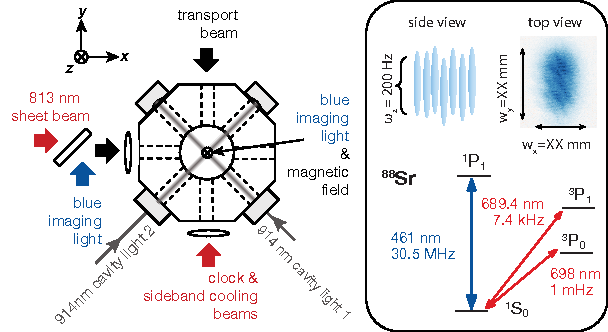
\includegraphics[]{figures/setup.pdf}
	    \caption{Optical setup}
	    \label{fig:setup}
	\end{figure}

	Our optical trap is generated by two-dimensional optical lattices created in the build-up cavities and a sheet-like dipole trap, as illustrated in Figure \ref{fig:setup}. Since the sheet beam is magic to the clock transition and its trap frequency is much smaller than the lattice trap frequencies ($\sim$ 200 Hz), we ignore the influence of the sheet beam for now. For the two-dimensional lattices, the potential is

	\begin{align}
	U(x,y,z)&=U^{x}_{0}\bigg(\frac{w_{0}}{w(x)}\bigg)^{2}e^{-2(y^{2}+z^{2})/w^{2}_{0}}\text{cos}^{2}(kx)+U^{y}_{0}\bigg(\frac{w_{0}}{w(y)}\bigg)^{2}e^{-2(x^{2}+z^{2})/w^{2}_{0}}\text{cos}^{2}(ky) \nonumber \\
	&\stackrel{x,y \approx 0}{\approx} U^{x}_{0}e^{-2(y^{2}+z^{2})/w^{2}_{0}}\text{cos}^{2}(kx)+U^{y}_{0}e^{-2(x^{2}+z^{2})/w^{2}_{0}}\text{cos}^{2}(ky) \nonumber\\
	&\stackrel{U_{x}=U_{y}, z\approx{0}}{\approx} U_{0}\bigg(e^{-2y^{2}/w^{2}_{0}}\text{cos}^{2}(kx)+e^{-2x^{2}/w^{2}_{0}}\text{cos}^{2}(ky)\bigg),
	\label{eq:2d_potential}
	\end{align}

	\noindent where $U^{i}_{0} = - \alpha_{i} I_{0} / (2c\epsilon_{0})$, $\alpha_{i}$ is polarizability of a state $i$, and $w_{0}$ is the waist of the cavity mode. In Equation \ref{eq:2d_potential}, we made the approximations $w_{0}/w(x)\approx1$ and $e^{-2z^{2}/w^{2}_{0}}\approx 1$, which are valid because the Rayleigh range of the cavities modes are $\sim 70$ cm and the sheet confines the atoms at the gravity compensated position where $z\approx 60 \ \mu \text{m} \ll  w_{0}$. The vibrational energy of the atoms trapped in the deep two-dimensional optical lattices ~\cite{blatt09} is

	\begin{align}\label{eq:2d_potential_vmode_energy}
	E_{n_x,n_y}&=h\nu_{x}(n_{x}+1/2)-h\frac{\nu_{\text{rec}}}{2}(n^{2}_{x}+n_{x}+1)
	+h\nu_{y}(n_{y}+1/2)-h\frac{\nu_{\text{rec}}}{2}(n^{2}_{y}+n_{y}+1) \nonumber\\
	&\stackrel{\nu_x=\nu_y}=h\nu + n_{xy}h\nu - h\frac{\nu_{\text{rec}}}{2}(n^{2}_x+n^{2}_y+n+2)
	\end{align}

	\noindent where $n_{i}$, $\nu_{\text{rec}}$, and $n_{xy}$ are vibrational mode along $i$ axis, recoil frequency, and $n_x+n_y$, respectively. Following Equation \ref{eq:2d_potential_vmode_energy}, the energies of $n_{00}=0$ or $n_{10}=1$ (or $n_{01}$) states are

	\begin{align}
	\begin{split}\label{eq:energy_deep_lattice_n0}
		& E_{0,0}=h\nu-h\nu_{\text{rec}}
	\end{split}\\
	\begin{split}\label{eq:energy_deep_lattice_n1}
		& E_{1,0}=2h\nu-2h\nu_{\text{rec}}
	\end{split}\\
	& \Delta E = h(\nu - \nu_{\text{rec}})\nonumber.
	% \label{eq:energy_deep_lattice}
	\end{align}


	\noindent So far, all the discussions have been the energies of a particular state in the trap. Now, let's look at the detuning required to drive the ground to excited states in the trap. This is particularly important for our purposes, since we are using this technique to characterize the cavity lattices. Since we are in non-magic lattices, we need to remember that the trap frequencies are different for the two states.

	% \begin{figure}
	%     \centering
	%     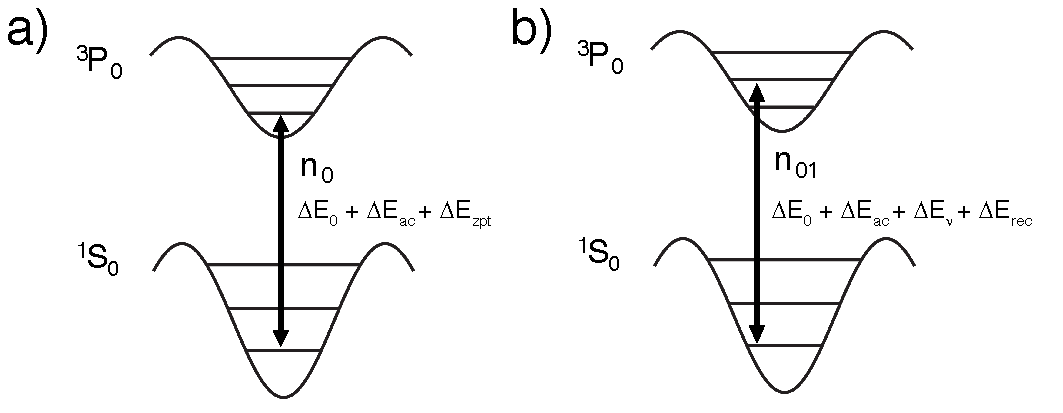
\includegraphics[scale=0.8]{figures/potential_intro.pdf}
	%     \caption{Energy required to drive carrier and sideband transitions}
	%     \label{fig:potential_intro}
	% \end{figure}


	In free space, the energy difference between $\SSZ (g)$ and $\TPZ (e)$ states is $\Delta E_{0}=\hbar\omega_{0}$. In non-magic lattices, there are additional energy shifts to consider: ac-Stark shift ($\Delta E_{\text{ac}}$) and a shift due to the vibrational mode energy difference ($\Delta E_\nu$). Let's first consider the energy required to drive a carrier transition $n^{g}_{00}\xleftrightarrow{}n^{e}_{00}$, where $n^{i}_{jk}$ specifies vibrational mode $jk$ of a state $i$, 

	\begin{align}
	\Delta E&=\Delta E_{0}+\Delta E_{\text{ac}} + \Delta E_{\nu} \nonumber\\ 
	&=\hbar\omega_0+ \frac{I(x,y)}{c\epsilon_0}(\alpha_g-\alpha_e)+h(\nu_e-\nu_g) \nonumber \nonumber\\
	&\approx\hbar\omega_0+ \frac{I(x,y)}{c\epsilon_0}(\alpha_g-\alpha_e)+
	\sqrt{\frac{2h\nu_{\text{rec}}I(x,y)}{c\epsilon_{0}}}(\sqrt{\alpha_e}-\sqrt{\alpha_g}),
	\label{eq:carrier_energy}
	\end{align}

	\noindent where $\alpha_{i}$ and $\nu_{i}$ are the polarizability and trap frequency of a state $i$, respectively. To calculate $\Delta E_{\nu}$, we use Equation \ref{eq:energy_deep_lattice_n0}. In the last step, we use $\nu_{\text{i}}\approx 2\sqrt{\nu_{\text{rec}}\abs{U_{i}}/h}$ where $U_{i}=-\alpha_{i}I(x,y)/2c\epsilon_0$, assuming the lattices with perfect contrasts. Rewriting Equation \ref{eq:carrier_energy}, the detuning required to drive a $n^{g}_{00}$ to $n^{e}_{00}$ is 

	% \begin{align*}
	% \delta&=\frac{I(x,y)}{2c\epsilon_0}(\alpha_g-\alpha_e)+h(\nu_e-\nu_g) \nonumber\\
	% &\approx \frac{I(x,y)}{2c\epsilon_0h}(\alpha_g-\alpha_e)+\sqrt{\frac{2\nu_{\text{rec}}I(x,y)}{c\epsilon_{0}h}}(\sqrt{\alpha_e}-\sqrt{\alpha_g}),\\
	% % \label{eq:detuning}
	% \end{align*}

	\begin{align}
	\delta&=\frac{\nu^{2}_g}{2\nu_{\text{rec}}}\bigg(1-\frac{\alpha_e}{\alpha_g}\bigg) + \nu_g\bigg(\sqrt{\frac{\alpha_e}{\alpha_g}}-1\bigg)
	\label{eq:carrier_freq_vg}
	\end{align}

	\noindent or writing in terms of $\nu_e$ instead, one arrives at 

	\begin{align}
	\delta&=\frac{\nu^{2}_e}{2\nu_{\text{rec}}}\bigg(\frac{\alpha_g}{\alpha_e}-1\bigg) + \nu_e\bigg(1-\sqrt{\frac{\alpha_g}{\alpha_e}}\bigg).
	\label{eq:carrier_freq_ve}
	\end{align}


	\noindent We can also look at $\Delta E$ required to drive a sideband transition $n^{g}_{ii} \xleftrightarrow{} n^{e}_{i,i+1}$


	\begin{align}
	\Delta E&=\Delta E_{0}+\Delta E_{\text{ac}} + \Delta E_{\nu} \nonumber \\ 
	&=\hbar\omega_0+ \frac{I(x,y)}{c\epsilon_0}(\alpha_g-\alpha_e)+h(\nu_e-\nu_{\text{rec}}) \nonumber \\
	&\approx\hbar\omega_0+ \frac{I(x,y)}{c\epsilon_0}(\alpha_g-\alpha_e)+h\bigg(\sqrt{\frac{2\nu_{\text{rec}}I(x,y)}{c\epsilon_0 h}}-\nu_{\text{rec}}\bigg),
	% \label{eq:sideband_energy}
	\end{align}

	\noindent where, again, the perfect contrast lattice assumption has been made in the last step. 

	% The maximum trap depth is 2$\abs{U_{0}}$ where $U_{0}=-\alpha_{\SSZ}I(0,0)/2c\epsilon_0$, and the maximum differential trap depth is 

	% \begin{align*}
	% \delta U_{\text{max}}=2U_{0}\bigg(1-\frac{\alpha_{e}}{\alpha_{g}}\bigg).
	% \end{align*}

	% \noindent For the perfect contrast lattices, one can get write $U_{\text{max}}$ in terms of $\nu_{g}$ and polarizability ratio $\alpha_g/\alpha_e$

	% \begin{align}
	% \delta U_{\text{max}}=2\bigg(\frac{h\nu^{2}_{g}}{4\nu_{\text{rec}}}\bigg)\bigg(1-\frac{\alpha_{e}}{\alpha_{g}}\bigg).
	% \end{align}


	% The energy required to drive a carrier transition ($n_{i,i}^{\SSZ} \xleftrightarrow{} n_{i,i}^{\TPZ}$ where $n^{k}_{i,j}$ indicates motional state $i,j$ of the state $k$$) is

	% \begin{align*}
 % 	\Delta E &= \Delta E_{0} + \Delta E_{\text{ac}} + \Delta E_{\text{zpt}}, \\
	% & = \hbar \omega_{0},
	% \end{align*}

	% \noindent where $E_{0}$, 

\subsection{Measurements}
	\subsubsection{Gaussian intensity profile}

		\begin{figure}
		    \centering
		    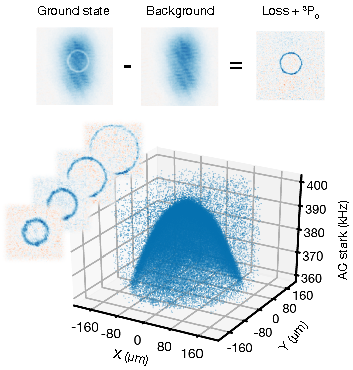
\includegraphics[scale=1.5]{figures/potential_map.pdf}
		    \caption{Reconstructed potential map (the quality of the figure is not great, will be updated later)}
		    \label{fig:potential_map}
		\end{figure}

		We can reconstruct the two-dimensional potential map as shown in Figure \ref{fig:potential_map} (will skip going into the details, since most of us are familiar with it). The fit function for the potential can be derived from Equation \ref{eq:carrier_energy}. So far, we have been neglecting $E_{v}$ term in Equation \ref{eq:carrier_energy} for the fit, since $E_{v} \ll E_{\text{ac}}$ ($\sim$ 10 kHz $\ll$ 400 kHz). Neglecting $E_{v}$ term, the fit function is 

		\begin{align*}
			\delta(x,y)=\frac{\delta_{\text{tot}}}{2+\epsilon}\bigg(e^{\frac{-2x}{w^{2}_{0}}}+(1+\epsilon)e^{\frac{-2y}{w^{2}_{0}}}\bigg)
		\end{align*}

		\noindent where $\epsilon$ characterizes the imbalance between the two orthogonal lattice axes' trap depths. The variables of the fit are the cavity mode waist $w_{0}$ and $\epsilon$. The total detuning $\delta_{\text{tot}}$ can be extracted separately from the ground or excited state trap frequency measurements (subsection \textbf{\nameref{subsection:trap_freq}}) or by beating the frequency comb and the clock laser (subsection \textbf{\nameref{subsection:comb}}).

	\subsubsection{Ground and excited state trap frequencies ($\alpha_{\text{g}}/\alpha_{\text{e}}$)}
		\label{subsection:trap_freq}

		In two-dimensional lattices which are not magic for the \SSZ (g) and \TPZ (e) states, the carrier transitions are resolved. As illustrated in Figure \ref{fig:trap_frequency_schematics}, by subtracting the carrier ($n^{g}_{00}\xleftrightarrow{} n^{e}_{00}$ or $n^{g}_{11}\xleftrightarrow{} n^{g}_{11}$) and blue sideband ($n^{g}_{00}\xleftrightarrow{} n^{e}_{10}$) transition frequencies, we can find ground and excited state trap frequencies. This can be easily derived from Equation \ref{eq:energy_deep_lattice_n0} and \ref{eq:energy_deep_lattice_n1}

		\begin{figure}
		    \centering
		    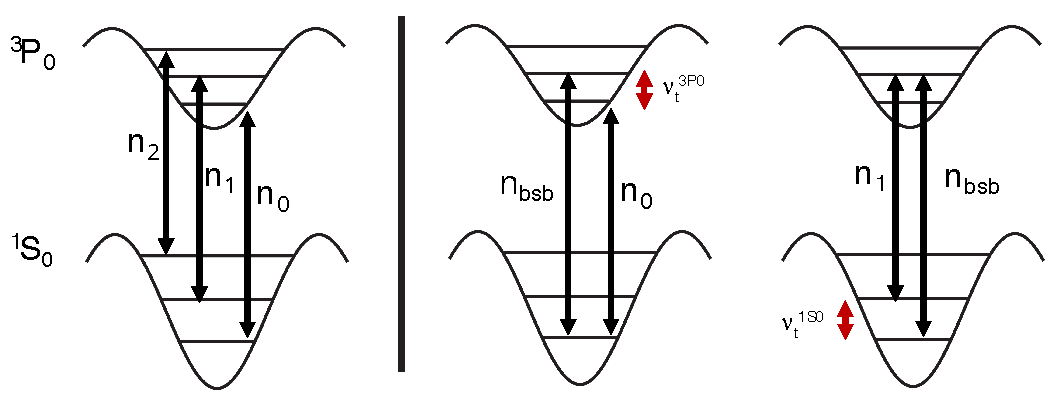
\includegraphics[scale=0.8]{figures/trap_frequency_schematics.pdf}
		    \caption{Carrier transitions are resolved (left) and by combining carrier and sideband transitions, one can find out ground and excited trap frequencies (right two pictures)}
		    \label{fig:trap_frequency_schematics}
		\end{figure}

			\begin{align*}
				\Delta f_{00,10}-\Delta f_{00,00}&=(E^{e}_{1,0}-E^{g}_{0,0})/h-(E^{e}_{0,0}-E^{g}_{0,0})/h \\
				&=(2\nu_e-2\nu_{\text{rec}}-\nu_g+\nu_{\text{rec}})-(\nu_e-\nu_{\text{rec}}-\nu_g+\nu_{\text{rec}}) \\		
				&=(2\nu_e-\nu_g-\nu_{\text{rec}})-(\nu_e-\nu_g) \\	
				&=\nu_e-\nu_{\text{rec}}
			\end{align*}
		and
			\begin{align*}
				\Delta f_{00,10}-\Delta f_{11,11}&=(E^{e}_{1,0}-E^{g}_{0,0})/h-(E^{e}_{1,0}-E^{g}_{1,0})/h \\
				&=(2\nu_e-2\nu_{\text{rec}}-\nu_g+\nu_{\text{rec}})-(2\nu_e-2\nu_{\text{rec}}-2\nu_g+2\nu_{\text{rec}}) \\		
				&=(2\nu_e-\nu_g)-(2\nu_e-2\nu_g) \\	
				&=\nu_g-\nu_{\text{rec}},
			\end{align*}

		\noindent where $f_{ij,kf}$ is the transition frequency from $n^{g}_{ij}\xleftrightarrow{} n^{g}_{kf}$.
		Figure \ref{fig:carrier_sideband_spectra} shows the carrier and sideband spectra for 2 by 2 averaged pixels. From the Lorentzian fits, we can find out $\Delta f_{00,00}$, $\Delta f_{11,11}$, and $\Delta f_{00,10}$. By subtracting the correct pairs, we can find out the polarizability ratio

		\begin{align}
			&\frac{\alpha_g}{\alpha_e}=\bigg(\frac{\Delta f_{00,10}-\Delta f_{11,11}+\nu_{\text{rec}}}{\Delta f_{00,10}-\Delta f_{00,00}+\nu_{\text{rec}}}\bigg)^{2}.
			\label{eq:ratio_extraction}
		\end{align}

		 \noindent Equation \ref{eq:ratio_extraction} was confirmed numerically (based on Sebastian's python code: lattice\_rings.py). The result is shown on the left in Figure \ref{fig:pol_ratio}, which clearly depicts that our estimation is susceptible to systemic errors. Ideally one would expect a flat distribution of the ratio across the sample; however, the ratio increases with the distance from the central pixel. So far, we are not sure what the cause is. If we ignore this systemic effect and restrict the estimation in a smaller central region (left on Figure \ref{fig:pol_ratio}), the noise distribution seems random. In this central area, the estimated ratio is \textbf{1.179 $\pmb{\pm}$ 0.002}. 

		\begin{figure}
		    \centering
		    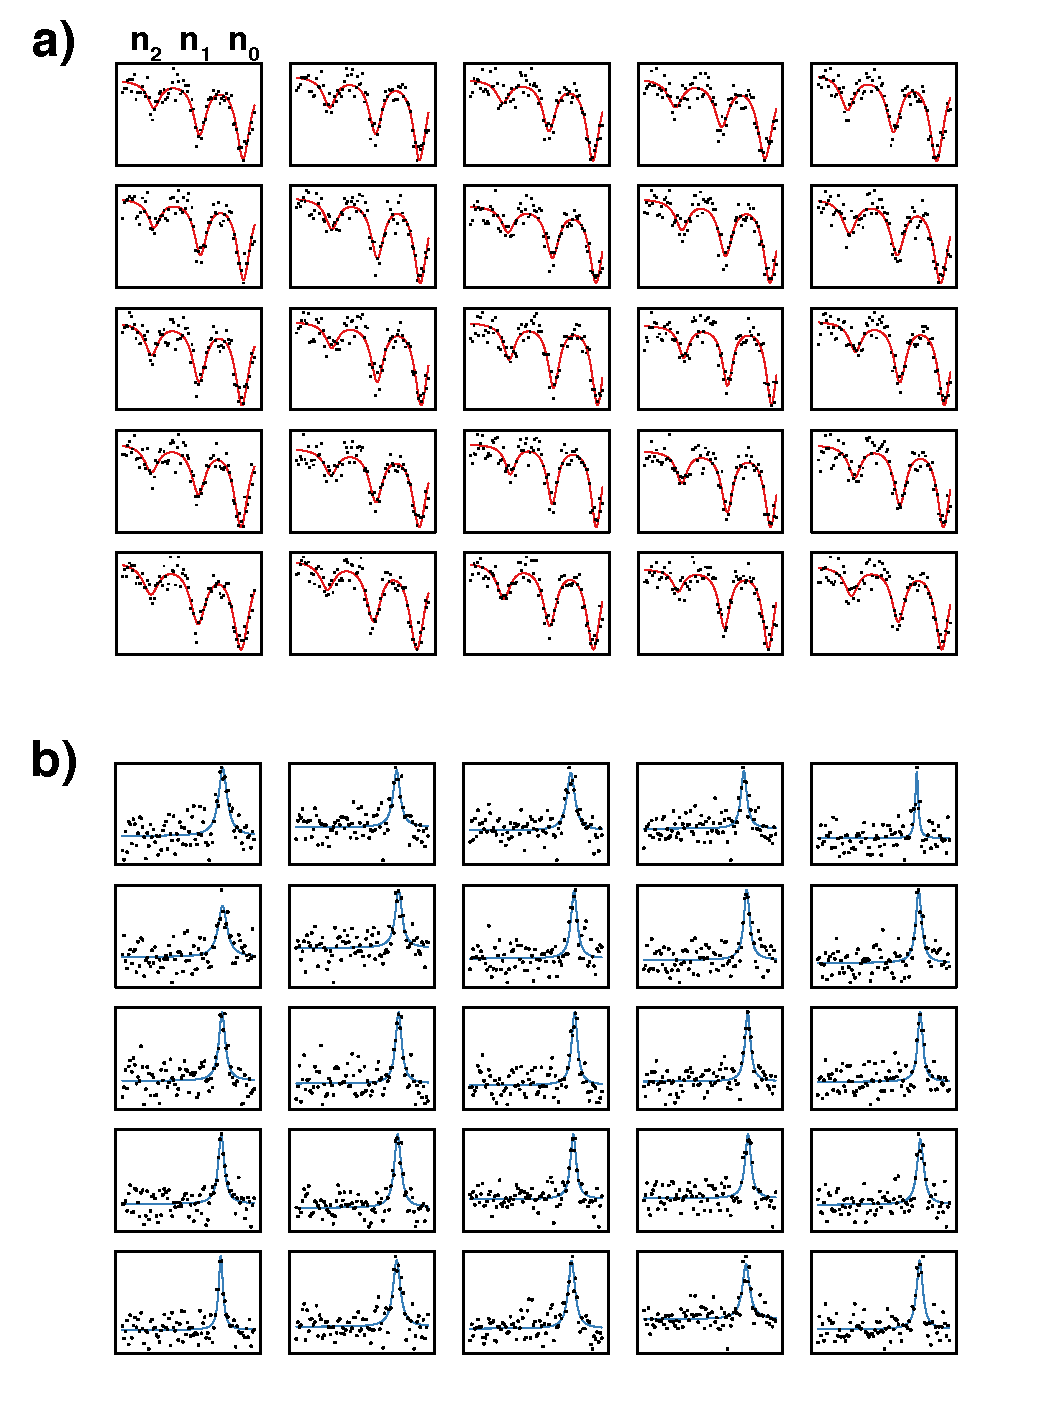
\includegraphics[scale=0.8]{figures/carrier_sideband_spectra.pdf}
		    \caption{Carrier sideband spectra, data folder: \textbackslash data \textbackslash\_2020\textbackslash10\textbackslash29\textbackslash it\_sr88\_clock\_fringe\\ \_arm1=1.175V\_arm2\_0.975V\_z\_cooling\_2 \& it\_sr88\_clock\_fringe\_arm1=1.175V\_arm2\_0.975V\_bluesideband\_fine}
		    \label{fig:carrier_sideband_spectra}
		\end{figure}

		\begin{figure}
		\hspace*{-2cm}
		\begin{subfigure}{0.4\linewidth}
			\includegraphics[scale=0.7]{figures/pol_ratio_size6.png}
		\end{subfigure}
		\qquad\qquad\qquad\quad
		\begin{subfigure}{0.4\linewidth}
			\includegraphics[scale=0.7]{figures/pol_ratio_size4.png}
		\end{subfigure}
		\caption{Polarizability $\alpha_g/\alpha_e$ ratio for (a) larger size (b) smaller size} 
		\label{fig:pol_ratio}
		\end{figure}


	\subsubsection{Absolute clock laser detuning}\label{subsection:comb}
			We measure the absolute clock laser detuning required to address the atoms in the center of the lattices by beating the frequency comb with the clock laser. The expected detuning as a function of trap frequency (intensity) is expressed in Equation \ref{eq:carrier_freq_vg} and \ref{eq:carrier_freq_ve} (Equation \ref{eq:carrier_energy}). The clock laser beam path is splitted into multiple paths as shown in Figure \ref{fig:clocklaser setup}, one of the paths is fiber coupled to the frequency comb setup, and the other path goes through a scanning double pass (DP) aom and then, fiber coupled to seed the injection lock. The output of the injection is used to probe the atoms.

		\begin{figure}
		    \centering
		    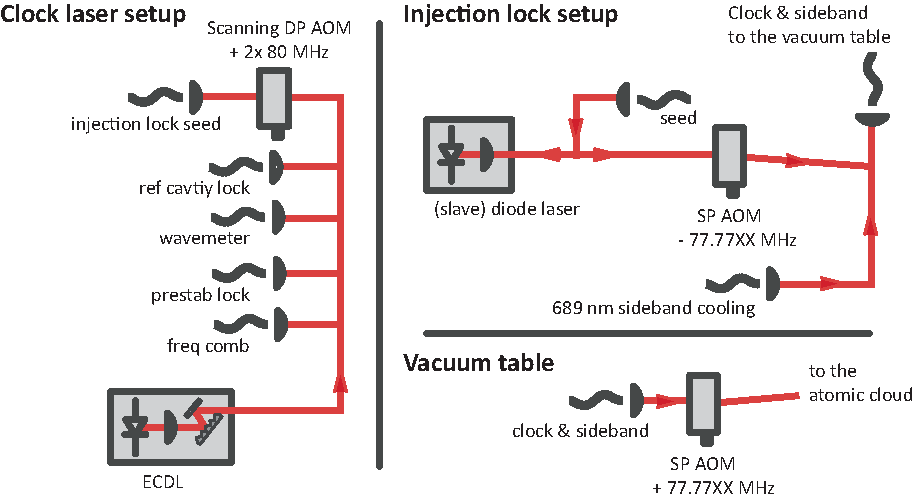
\includegraphics[scale=0.8]{figures/clocklaser_setup.pdf}
		    \caption{Clocklaser setup}
		    \label{fig:clocklaser setup}
		\end{figure}

			To measure the maximum light shift, we scanned the double pass aom frequency to excite the center of the lattices. We repeated these measurements for two different trap frequencies. Figure \ref{fig:total_ac_stark_spectrum} shows the carrier and blue sideband spectra. Taking each spectrum takes about half an hour to an hour, and after each carrier scan, we recorded the beat frequency recorded on the counter to find out the absolute ac-Stark shift.

			The detunings with respect to the known $^{\text{88}}{\text{Sr}}$ \SSZ - \TPZ transition frequency~\cite{sansonetti10} were,


			\begin{itemize}
			  \item (399533 $\pm$ 400) Hz for "high depth"
			  \item (195385 $\pm$ 400) Hz for "half depth"
			\end{itemize}


			We know that the clock laser drifts about -400 Hz per hour. During the carrier frequency measurements, the DP aom frequeny has been compensating for the drift, whereas the fiber port that was used for the beat does not go through this DP aom, thus, susceptible for the drift. If we include this shift, 

			\begin{itemize}
			  \item (399533 $\pm$ 400 + 400) Hz for "high depth"
			  \item (195385 $\pm$ 400 + 400) Hz for "half depth"
			\end{itemize}

		% \begin{figure*}
		% \centering 
		% \includegraphics[scale=0.5]{figures/high_depth66_88.pdf}\qquad\quad
		% \includegraphics[scale=0.5]{figures/half_depth66_88.pdf}\par\medskip
		% \includegraphics[width=\textwidth]{figures/insitu_images.pdf}
		% \caption{}
		% \end{figure*}

			\begin{figure}
			\centering 
			\begin{subfigure}[b]{0.4\linewidth}
				\includegraphics[scale=0.5]{figures/high_depth66_88.pdf}
				\caption{}
			\end{subfigure}
			\qquad\qquad
			\begin{subfigure}[b]{0.4\linewidth}
				\includegraphics[scale=0.5]{figures/half_depth66_88.pdf}
				\caption{}
			\end{subfigure}

			\begin{subfigure}{\linewidth}
				\includegraphics[scale=0.4]{figures/insitu_images.pdf}
				\caption{}
			\end{subfigure}
			\caption{\textbf{(a)} carrier (top) and sideband (bottom) clock spectra of ground and excited states of high depth \textbf{(b)} same as (a) for half of the depth \textbf{(c)} in-situ \SSZ images at the center frequency of carrier and sideband spectra (data folder: \textbackslash data \textbackslash\_2020\textbackslash12\textbackslash02\textbackslash it\_sr88\_absolute\_ac\_stark)} 
			\label{fig:total_ac_stark_spectrum}

			\end{figure}


			\noindent Quadratic zeeman shift is about $\sim$ 1 kHz at 50 G that was used for the measurements. 

		% The spacing between $f_{00}$ and $f_{11}$ transition is 


		% 	\begin{align*}
		% 		f_{00}-f_{11}&=(E^{e}_{0,0}-E^{g}_{0,0})/h-(E^{e}_{1,1}-E^{g}_{1,1})/h \\
		% 		&=(\nu_e-\nu_{\text{rec}}-\nu_g+\nu_{\text{rec}})-(2\nu_e-2\nu_{\text{rec}}-2\nu_g+2\nu_{\text{rec}}) \\
		% 		&=(\nu_e-\nu_g)-(2\nu_e-2\nu_g) \\
		% 		&=\nu_g-\nu_e \\
		% 	\end{align*}


		% One can also look at the spacing between the $n_{00}$ and $n_{10}$ transitions which is related to $f_{n_{00}}-f_{n_{11}}=h(\nu_{\text{g}}-\nu_{\text{e}})=h\nu_{\text{g}}(1-\sqrt{\frac{\alpha_e}{\alpha_g}})$. 



		% Alternatively, one can measure the ratio of ground and excited polarizability:

		% \begin{align*}

		% \end{align*}

	% \subsection{Waist measurements}




	% \subsection{temperature}

\subsection{Cross-check}
	\subsubsection{Discrepancies between total ac-Stark \& Trap frequency measurements}

		We compare the measured polarizability ratio with the ratio derived using Marianna's polarizability values, which are (261.09 $\pm$ 1.16) a.u. at 914.0 nm and (260.91 $\pm$ 1.16) a.u. at 915.0 nm for $\alpha_g$, and (220.8 $\pm$ 2.3) a.u. at 914.332 nm for $\alpha_e$. To find out the $\alpha_g$ at 914.332 nm, I do linear interpolation and get (261.03 $\pm$ 0.87) at 914.332 nm. The comparisons with our measurement and Marianna's number are shown in Figure \ref{fig:ratio_comparison_plot} on left.

		\begin{figure}
		    % \centering
		    \hspace*{-0.5cm}
		    \includegraphics[scale=0.6]{figures/ratio_comparison_plot.pdf}
		    \caption{\textbf{(left)} polarizability ratio ($\alpha_g/\alpha_e$) comparison: M (Marianna's number) and measured \textbf{(middle)}: $\delta_{\text{tot}}$ comparison for the "high depth" data \textbf{(right)} $\delta_{\text{tot}}$ comparison for the "half depth" data}
		    \label{fig:ratio_comparison_plot}
		\end{figure}

		\noindent From the extracted ratio, we can cross check whether the comb measurement in Section \ref{subsection:comb} agrees with the trap frequency measurements performed on the same day (Figure \ref{fig:total_ac_stark_spectrum} (a) and (b)). For this cross check, we compare the total detuning $\delta_{\text{tot}}$ from the comb against the one derived from Equation \ref{eq:carrier_freq_ve}:

		\begin{align*}
		\delta_{\text{tot}}=\frac{\overbrace{\nu^{2}}^{\text{data: Fig. \ref{fig:total_ac_stark_spectrum}}}_e}{2\nu_{\text{rec}}}\bigg(\underbrace{\frac{\alpha_g}{\alpha_e}}_{\text{data: Fig. \ref{fig:carrier_sideband_spectra}}}-1\bigg) + \overbrace{\nu_e}^{\text{data: Fig. \ref{fig:total_ac_stark_spectrum}}}\bigg(1-\underbrace{\sqrt{\frac{\alpha_g}{\alpha_e}}}_{\text{data: Fig. \ref{fig:carrier_sideband_spectra}}}\bigg).
		\end{align*}

		The result is shown in Figure \ref{fig:ratio_comparison_plot}, which shows the discrepancies between the two results. Yet, we are not sure where the discrepancy is coming from.

		\paragraph{Can we extract $\alpha_g$?}
			The answer is no. From the two separate data sets, we extracted the polarizability ratio ($\alpha_g/\alpha_e$) and $\delta_{\text{tot}}$ at a particular $\nu_e$. It seems that by using Equation \ref{eq:carrier_freq_ve}, we should be able figure out $\alpha_g$ or $\alpha_e$. However, we cannot because the trap frequency depends on two parameters, polarizability and intensity ($I(x,y)$):

			\begin{align*}
				\nu_i=2\sqrt{\frac{\nu_{\text{rec}}\alpha_i I(x,y)}{2c\epsilon_0}}.
			\end{align*}

			\noindent Without a good knowledge of intensity, one cannot extract the polarizability. 
\section{Appendices}
\label{sec:appendices}
\subsection{Magnetic field calibration}
		
		\begin{figure}[h]
		    \centering
		    \includegraphics[scale=0.8]{figures/field_calibration.pdf}
		    \caption{\TPO m=1 transition frequency shift as a function of field set voltage datapath:\textbackslash data \textbackslash\_2020\textbackslash10\textbackslash26\textbackslash it\_field\_calibration}
		    \label{fig:field_calibration}
		\end{figure}

		\begin{figure}
		    \centering
		    \includegraphics[scale=0.8]{figures/field_calib_curve.pdf}
		    \caption{field calibration curve}
		    \label{fig:field_calib_curve}
		\end{figure}

\subsection{Clock laser waist calibration}
\subsection{Quadratic Zeeman Shift}

		\begin{figure}
		\centering
		\label{fig:qz}
		\begin{subfigure}{0.4\linewidth}
		    \includegraphics[scale=0.4]{figures/qz_spectrum.pdf}
		    \caption{clock resonant frequency shift for different field}
		\end{subfigure}
		\begin{subfigure}{0.4\linewidth}
		    \includegraphics[scale=0.4]{figures/quadratic_zeeman_shift.pdf}
		    \caption{Quadratic zeeman shift}
		\end{subfigure}
		\caption{}
		\end{figure}


		% \begin{figure}
		% % \centering 
		% \hspace*{-2cm}
		% \label{fig:pol_ratio}
		% \begin{subfigure}{0.4\linewidth}
		% 	\includegraphics[scale=0.7]{figures/pol_ratio_size6.png}
		% 	% \caption{}
		% \end{subfigure}
		% \qquad\qquad\qquad\quad
		% \begin{subfigure}{0.4\linewidth}
		% 	\includegraphics[scale=0.7]{figures/pol_ratio_size4.png}
		% 	% \caption{}
		% \end{subfigure}
		% \caption{Polarizability $\alpha_g/\alpha_e$ ratio for (a) larger size (b) smaller size} 
		% \end{figure}

			% \begin{figure}
			% \centering 
			% \begin{subfigure}[b]{0.4\linewidth}
			% 	\includegraphics[scale=0.5]{figures/high_depth66_88.pdf}
			% 	\caption{}
			% \end{subfigure}
			% \qquad\qquad
			% \begin{subfigure}[b]{0.4\linewidth}
			% 	\includegraphics[scale=0.5]{figures/half_depth66_88.pdf}
			% 	\caption{}
			% \end{subfigure}

			% \begin{subfigure}{\linewidth}
			% 	\includegraphics[scale=0.4]{figures/insitu_images.pdf}
			% 	\caption{}
			% \end{subfigure}
			% \caption{\textbf{(a)} carrier (top) and sideband (bottom) clock spectra of ground and excited states of high depth \textbf{(b)} same as (a) for half of the depth \textbf{(c)} in-situ \SSZ images at the center frequency of carrier and sideband spectra (data folder: \textbackslash data \textbackslash\_2020\textbackslash12\textbackslash02\textbackslash it\_sr88\_absolute\_ac\_stark)} 
			% \label{fig:total_ac_stark_spectrum}

			% \end{figure}


\subsection{Ac-Stark shift from the clock laser}
	very small
% \subsection{Magnetic field calibration}
% \subsection{Probe intensity calibration}

\bibliography{main}{}
\bibliographystyle{plain}




\end{document}
